\chapter{NAT (Dynamic): Part 2}\label{nat-dynamic-part-2}

\section{More About Static NAT}\label{more-about-static-nat}

\begin{itemize}
\tightlist
\item
  STATIC NAT involves statically configuring one-to-one mappings of
  PRIVATE IP ADDRESSES to PUBLIC IP ADDRESSES
\item
  When traffic from the INTERNAL HOST is sent to the OUTSIDE NETWORK,
  the ROUTER will translate the SOURCE ADDRESS
\end{itemize}

\begin{figure}
\centering
\pandocbounded{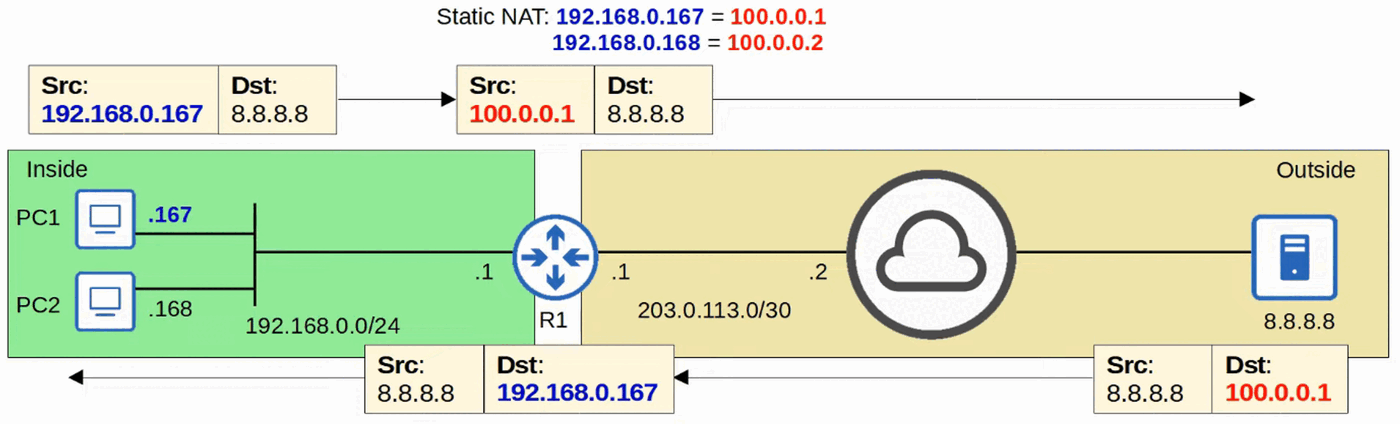
\includegraphics[keepaspectratio,alt={image}]{images/46-nat-dynamic-part2/img-001.png}}
\end{figure}

\begin{itemize}
\tightlist
\item
  HOWEVER, this one-to-one mapping also allows EXTERNAL HOSTS to access
  the INTERNAL HOST via INSIDE GLOBAL ADDRESS
\end{itemize}

\begin{figure}
\centering
\pandocbounded{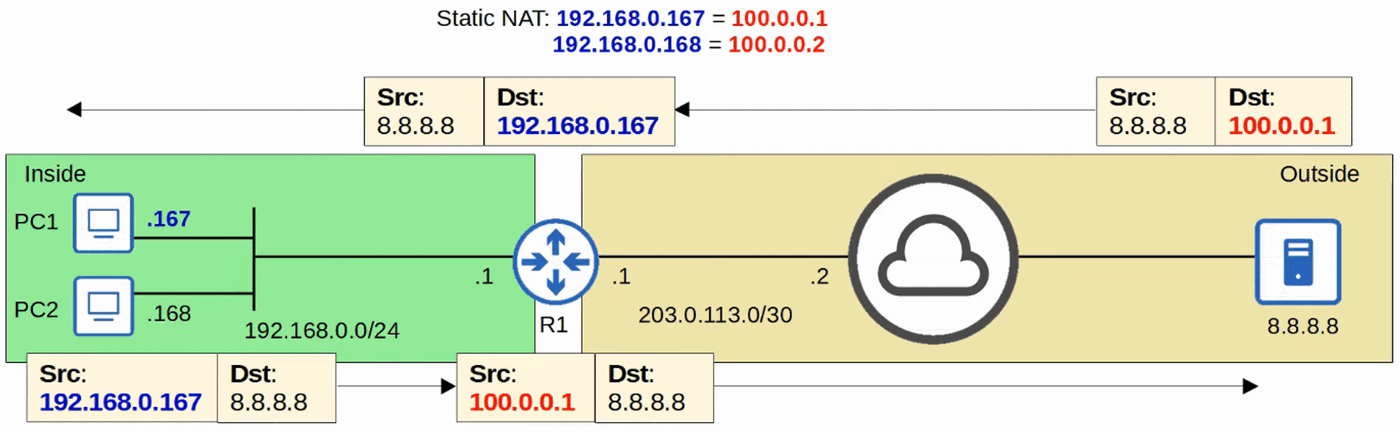
\includegraphics[keepaspectratio,alt={image}]{images/46-nat-dynamic-part2/img-002.png}}
\end{figure}

\section{Dynamic NAT}\label{dynamic-nat}

\begin{itemize}
\tightlist
\item
  In DYNAMIC NAT, the ROUTER dynamically maps INSIDE LOCAL ADDRESSES to
  INSIDE GLOBAL ADDRESSES, as needed
\item
  An ACL is used to identify WHICH traffic should be translated

  \begin{itemize}
  \tightlist
  \item
    If the SOURCE IP is PERMITTED; the SOURCE IP will be translated
  \item
    If the SOURCE IP is DENIED; the SOURCE IP will NOT be translated
  \end{itemize}
\end{itemize}

\begin{tipbox}

However, Packet Traffic will NOT be dropped

\end{tipbox}

\begin{itemize}
\tightlist
\item
  A NAT POOL is used to define the available INSIDE GLOBAL ADDRESS
\end{itemize}

\begin{figure}
\centering
\pandocbounded{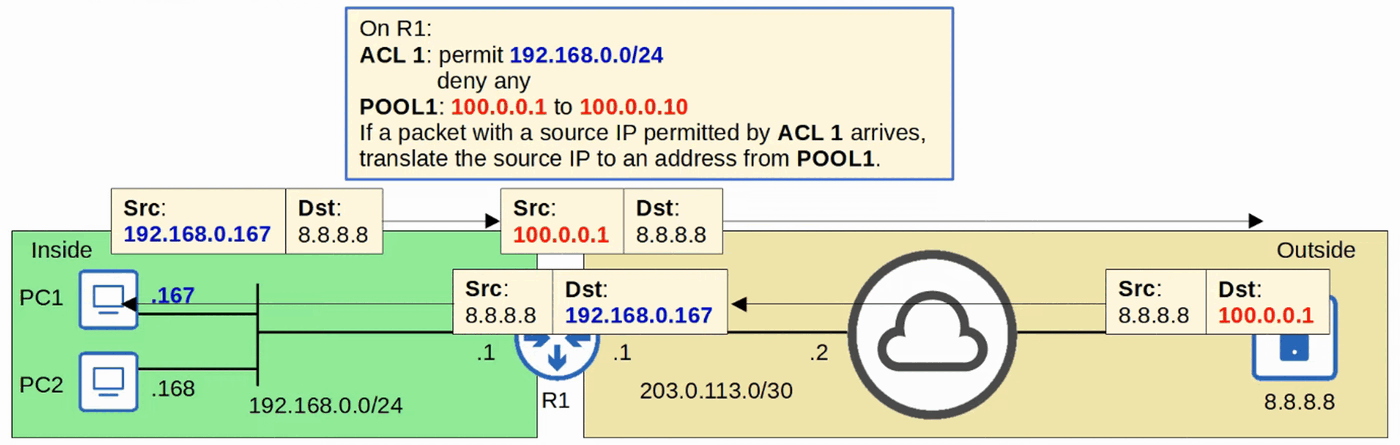
\includegraphics[keepaspectratio,alt={image}]{images/46-nat-dynamic-part2/img-003.png}}
\end{figure}

\begin{itemize}
\tightlist
\item
  Although they are dynamically assigned, the mappings are still
  one-to-one (one INSIDE LOCAL IP ADDRESS per INSIDE GLOBAL IP ADDRESS)
\item
  If there are NOT enough INSIDE GLOBAL IP ADDRESSES available (=ALL are
  being used), it is called `NAT POOL EXHAUSTION'

  \begin{itemize}
  \tightlist
  \item
    If a PACKET from another INSIDE HOST arrives and needs NAT but there
    are no AVAILABLE ADDRESSES, the ROUTER will drop the PACKET
  \item
    The HOST will be unable to access OUTSIDE NETWORKS until one of the
    INSIDE GLOBAL IP ADDRESSES becomes available
  \item
    DYNAMIC NAT entries will time out automatically if not used, or you
    can clear them manually
  \end{itemize}
\end{itemize}

\section{NAT Pool Exhaustion}\label{nat-pool-exhaustion}

\begin{figure}
\centering
\pandocbounded{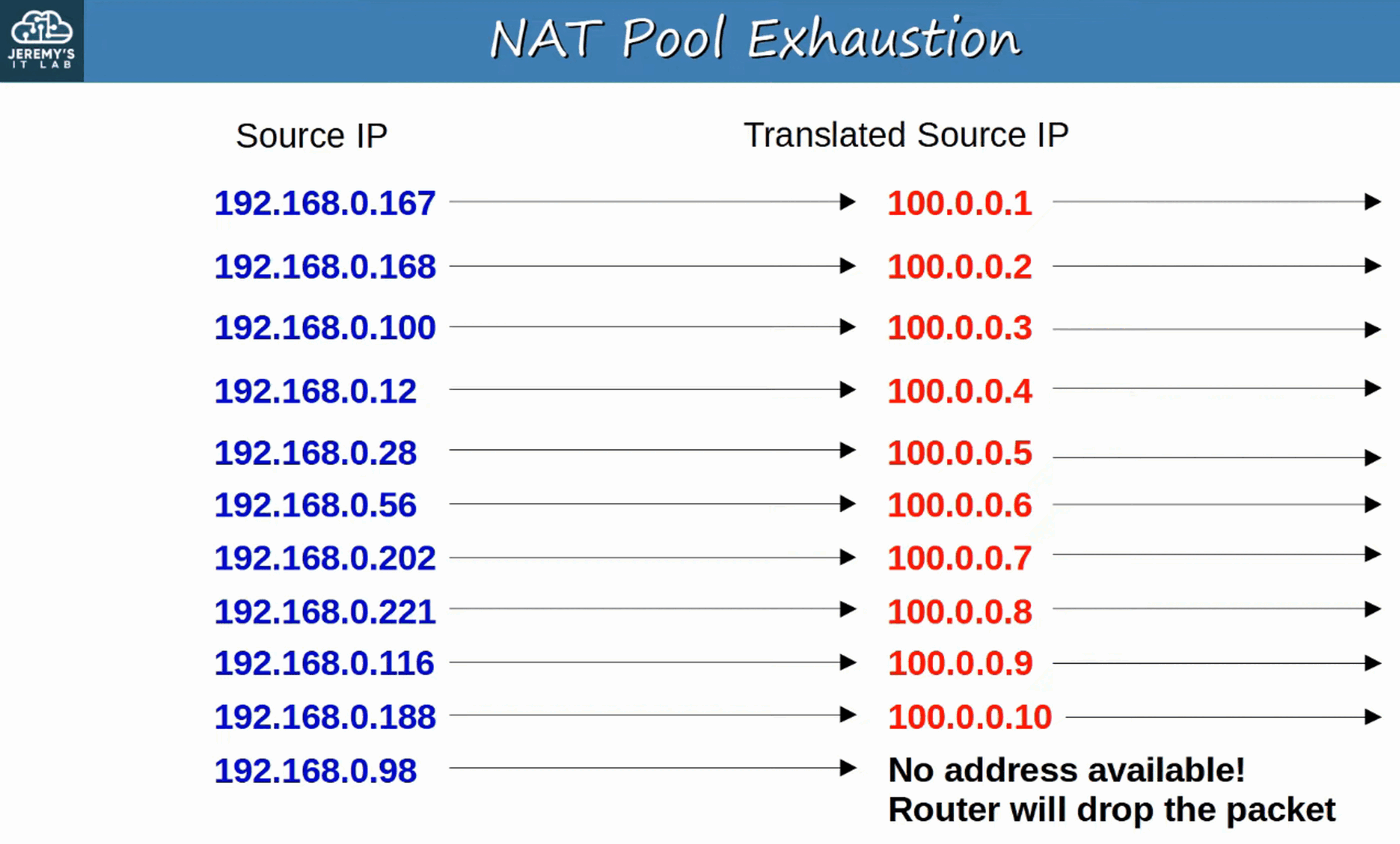
\includegraphics[keepaspectratio,alt={image}]{images/46-nat-dynamic-part2/img-004.png}}
\end{figure}

192.168.0.167 TIMES OUT and 192.168.0.98 is assigned it's TRANSLATED
SOURCE IP

\begin{figure}
\centering
\pandocbounded{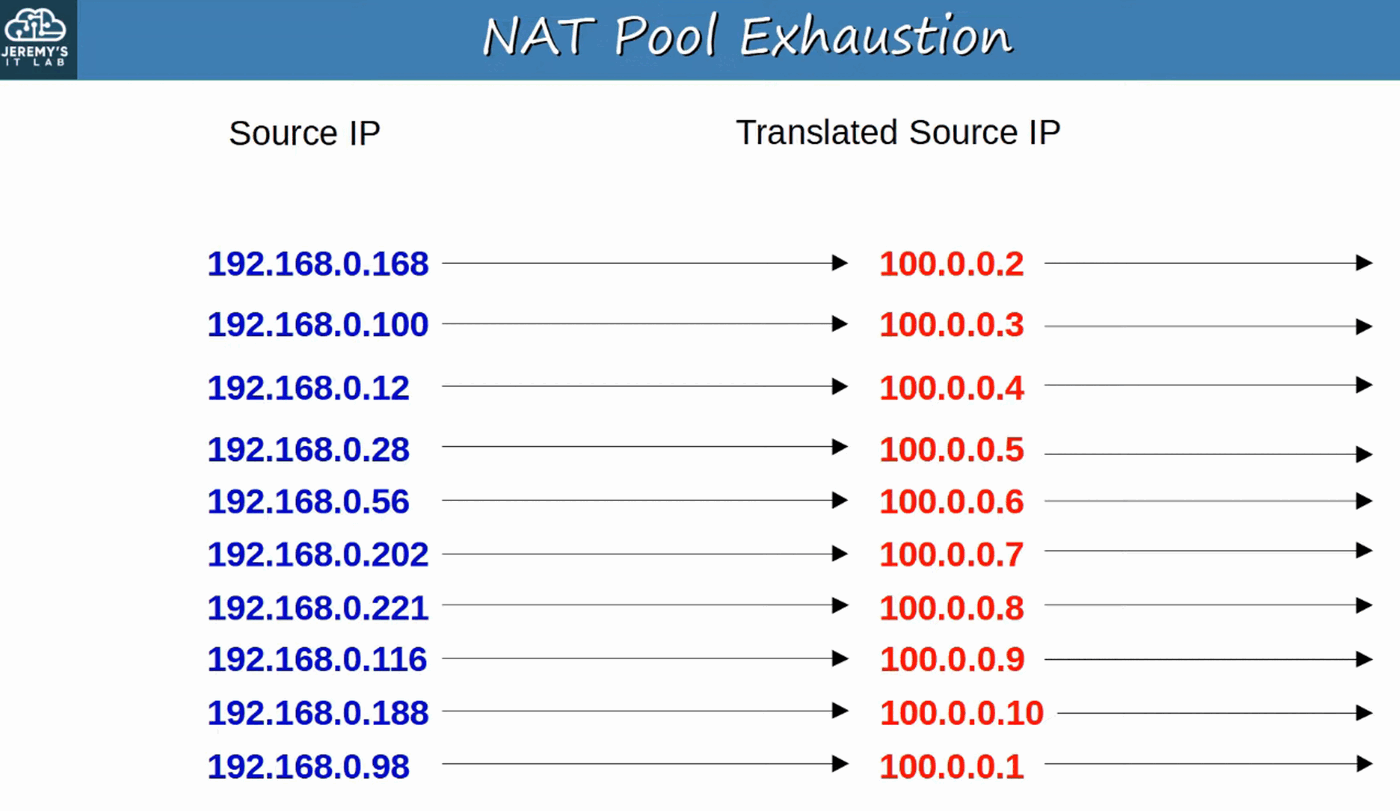
\includegraphics[keepaspectratio,alt={image}]{images/46-nat-dynamic-part2/img-005.png}}
\end{figure}

\section{Dynamic NAT Configuration}\label{dynamic-nat-configuration}

\begin{figure}
\centering
\pandocbounded{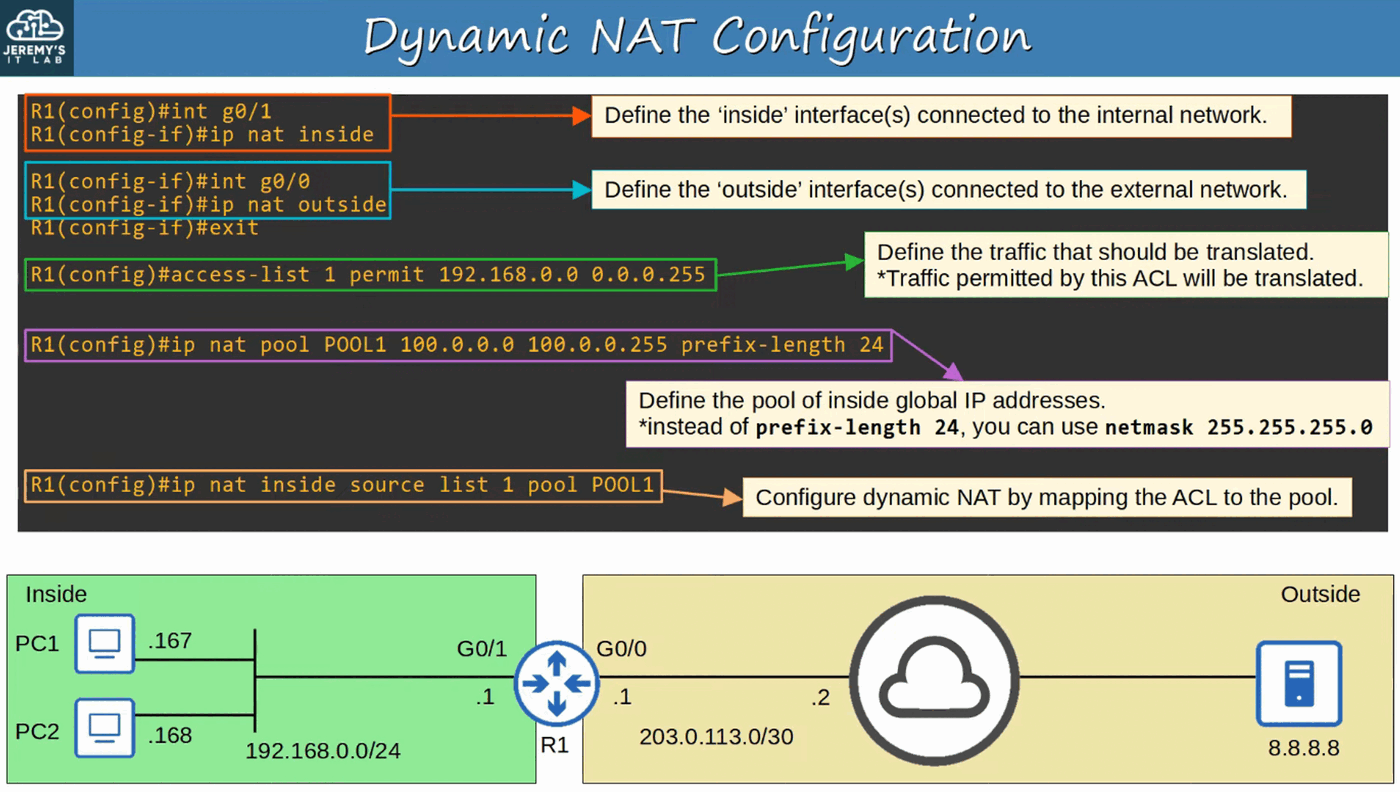
\includegraphics[keepaspectratio,alt={image}]{images/46-nat-dynamic-part2/img-006.png}}
\end{figure}

\passthrough{\lstinline!show ip nat translations!}

\begin{figure}
\centering
\pandocbounded{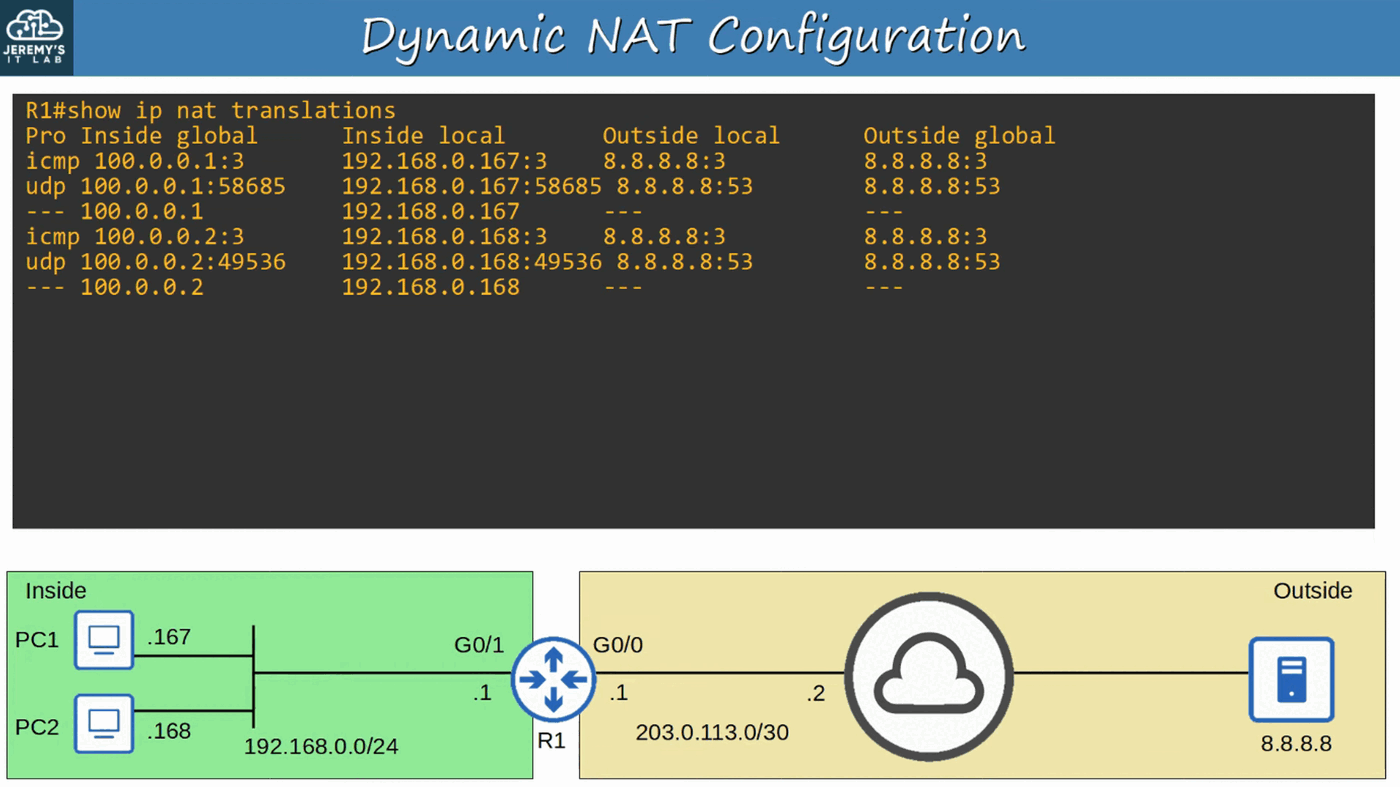
\includegraphics[keepaspectratio,alt={image}]{images/46-nat-dynamic-part2/img-007.png}}
\end{figure}

\begin{figure}
\centering
\pandocbounded{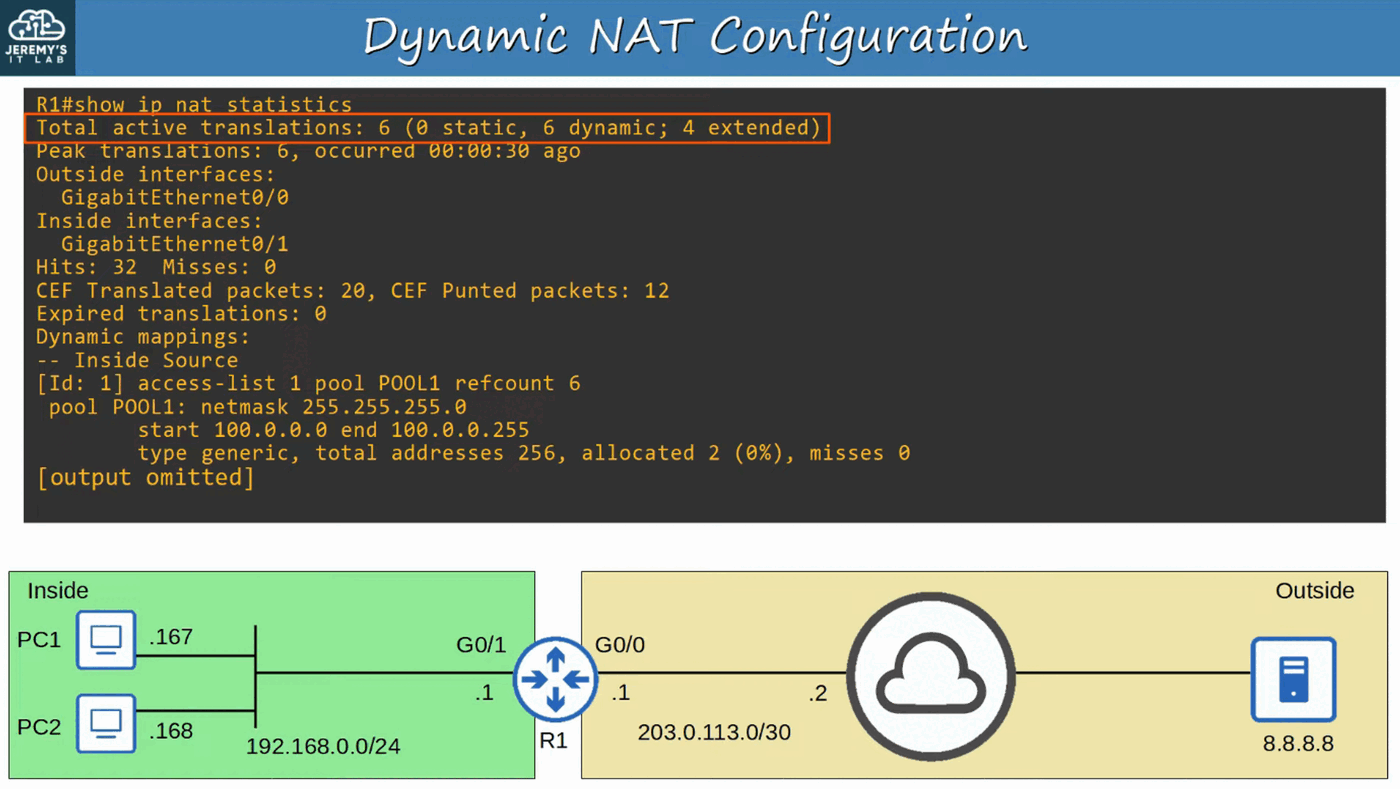
\includegraphics[keepaspectratio,alt={image}]{images/46-nat-dynamic-part2/img-008.png}}
\end{figure}

\begin{figure}
\centering
\pandocbounded{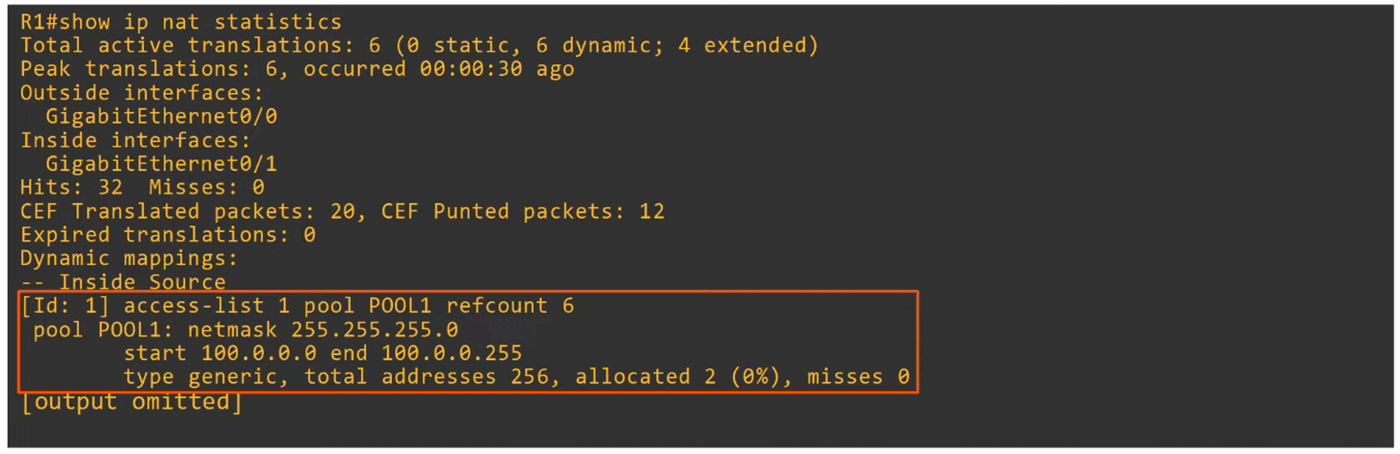
\includegraphics[keepaspectratio,alt={image}]{images/46-nat-dynamic-part2/img-009.png}}
\end{figure}

\section{Dynamic PAT (NAT Overload)}\label{dynamic-pat-nat-overload}

\begin{itemize}
\tightlist
\item
  PAT (NAT OVERLOAD) translates BOTH the IP ADDRESS and the PORT NUMBER
  (if necessary)
\item
  By using a unique PORT NUMBER for each communication flow, a single
  PUBLIC IP ADDRESS can be used by many different INTERNAL HOSTS

  \begin{itemize}
  \tightlist
  \item
    PORT NUMBERS are 16 bits = over 65,000 available port numbers
  \end{itemize}
\item
  The ROUTER will keep track of which INSIDE LOCAL ADDRESS is using
  which INSIDE GLOBAL ADDRESS and PORT
\end{itemize}

\begin{figure}
\centering
\pandocbounded{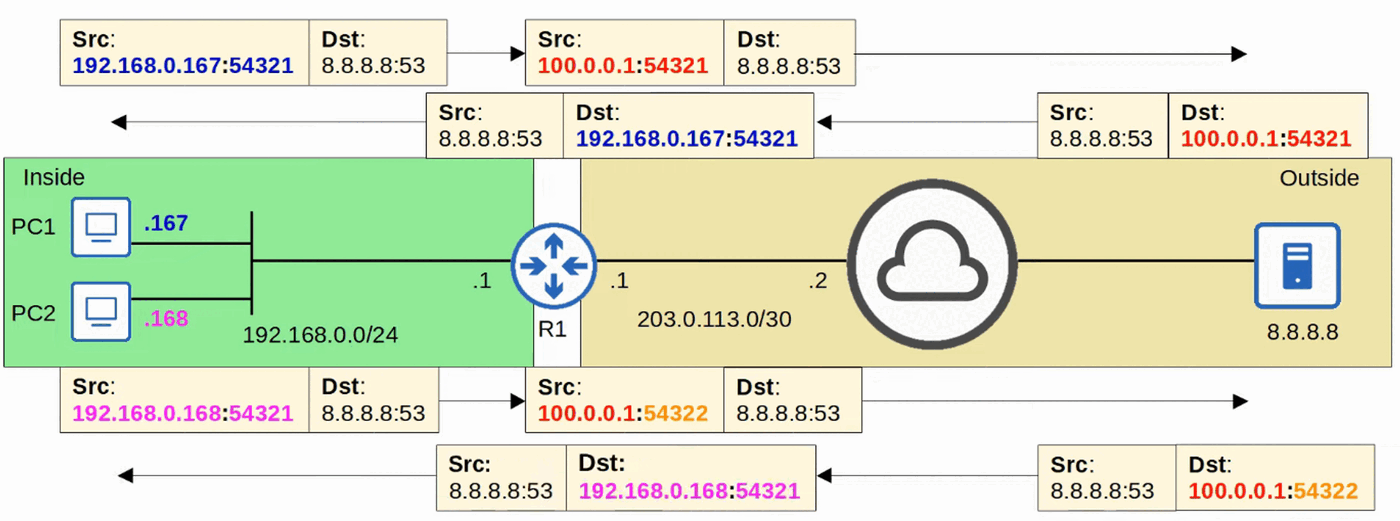
\includegraphics[keepaspectratio,alt={image}]{images/46-nat-dynamic-part2/img-010.png}}
\end{figure}

\section{PAT Configuration (Pool)}\label{pat-configuration-pool}

\begin{figure}
\centering
\pandocbounded{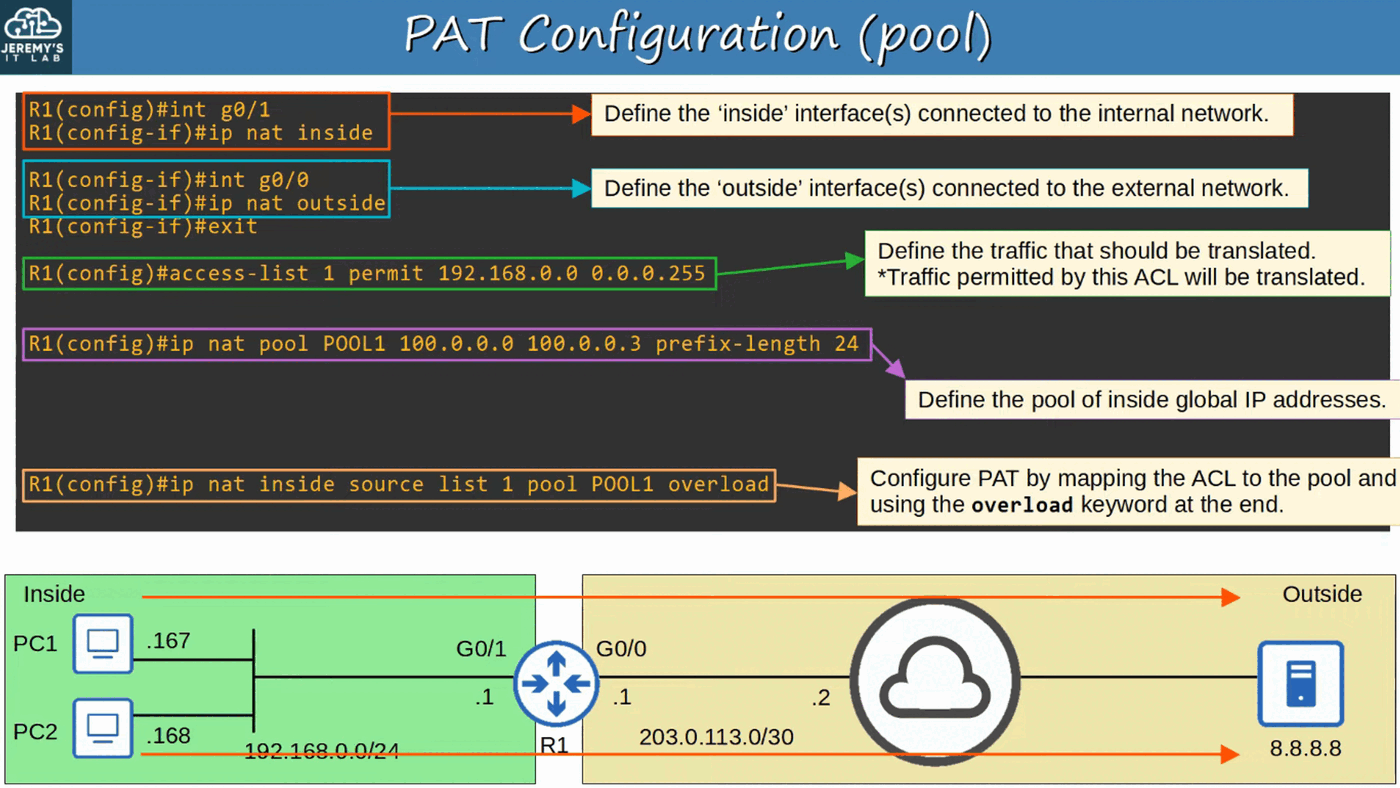
\includegraphics[keepaspectratio,alt={image}]{images/46-nat-dynamic-part2/img-011.png}}
\end{figure}

\passthrough{\lstinline!show ip nat translations!}

\begin{figure}
\centering
\pandocbounded{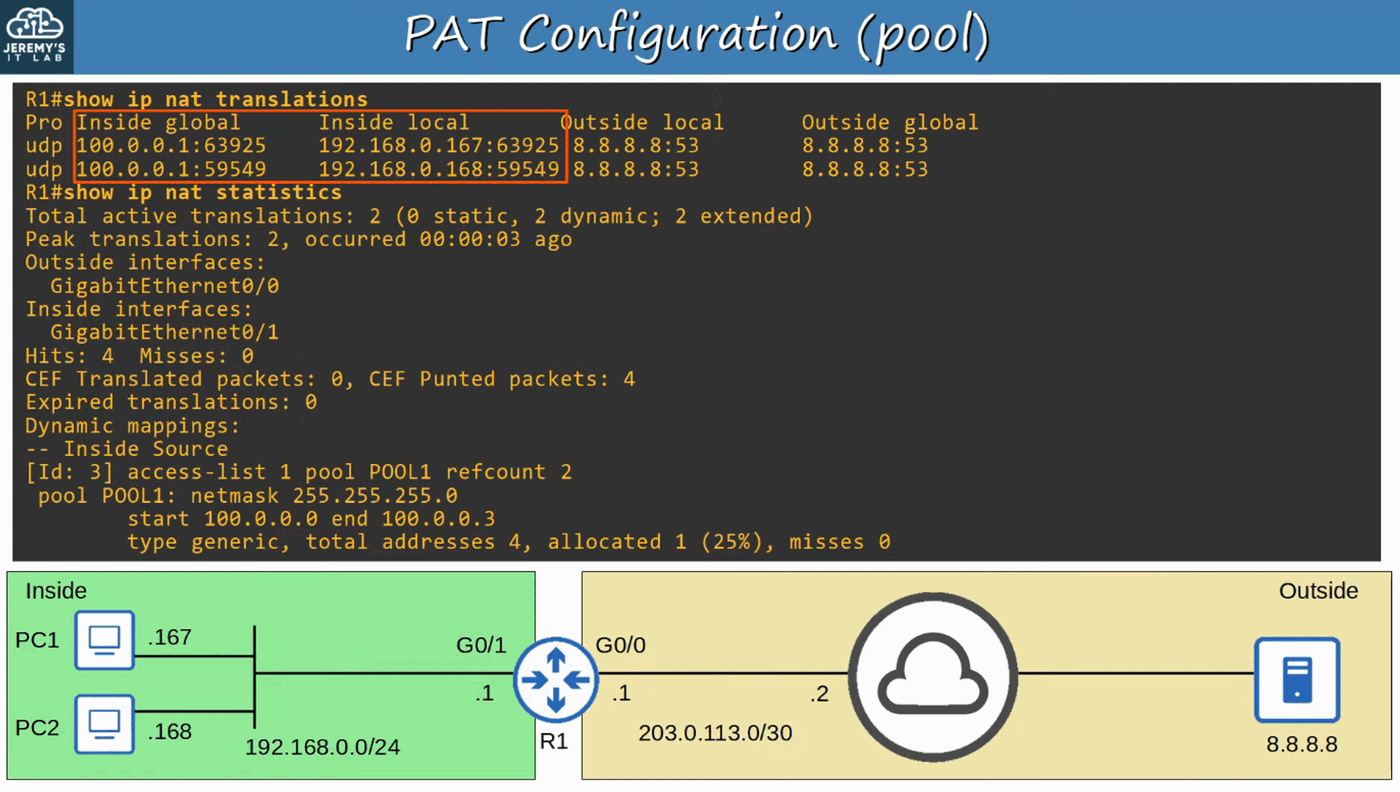
\includegraphics[keepaspectratio,alt={image}]{images/46-nat-dynamic-part2/img-012.png}}
\end{figure}

\section{PAT Configuration
(Interface)}\label{pat-configuration-interface}

\begin{figure}
\centering
\pandocbounded{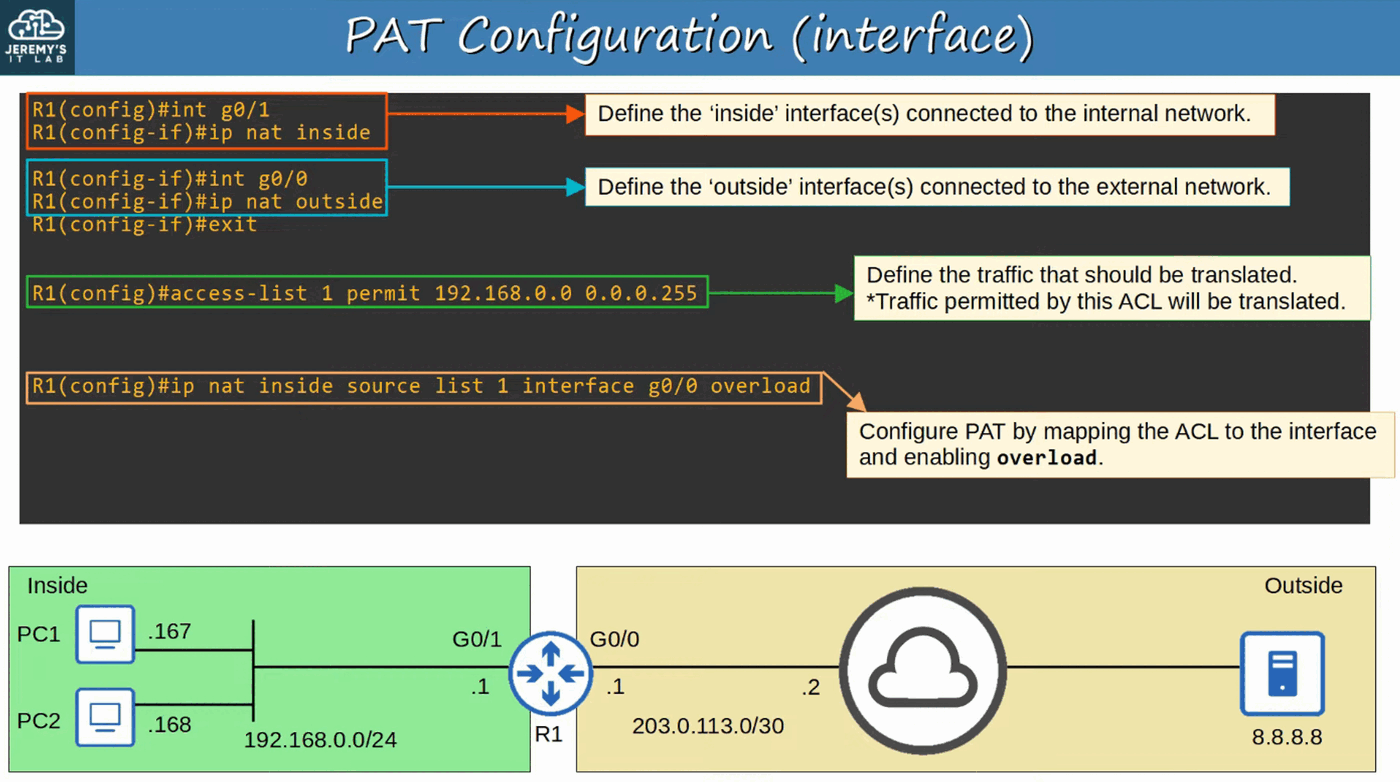
\includegraphics[keepaspectratio,alt={image}]{images/46-nat-dynamic-part2/img-013.png}}
\end{figure}

\begin{figure}
\centering
\pandocbounded{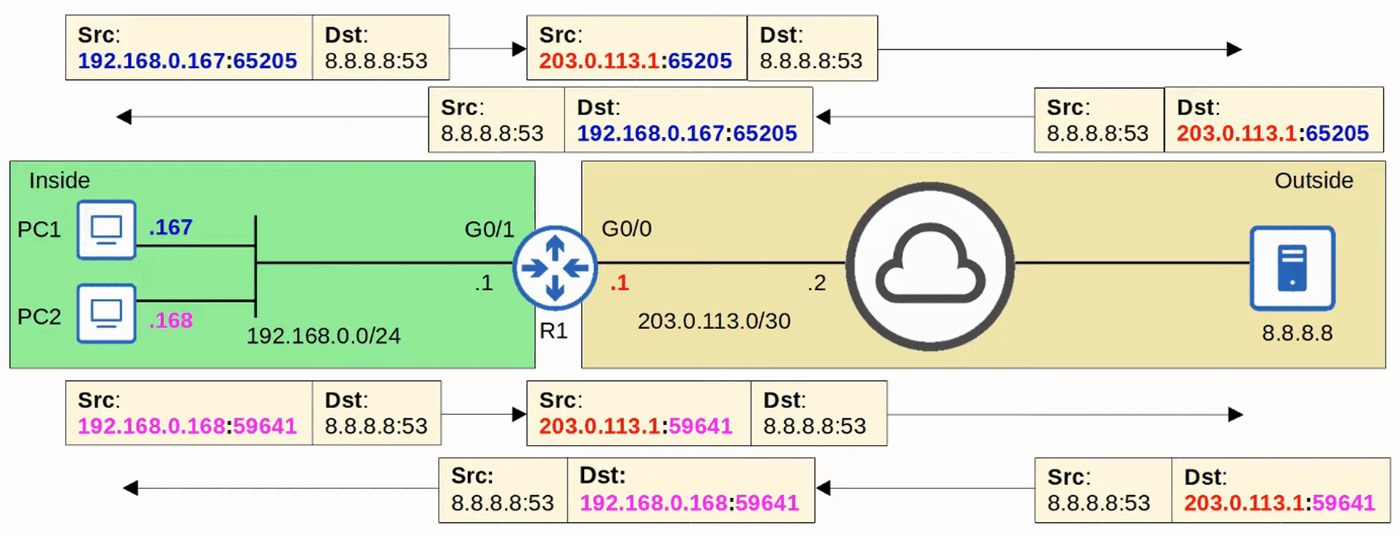
\includegraphics[keepaspectratio,alt={image}]{images/46-nat-dynamic-part2/img-014.png}}
\end{figure}

\passthrough{\lstinline!show ip nat translations!}

\begin{figure}
\centering
\pandocbounded{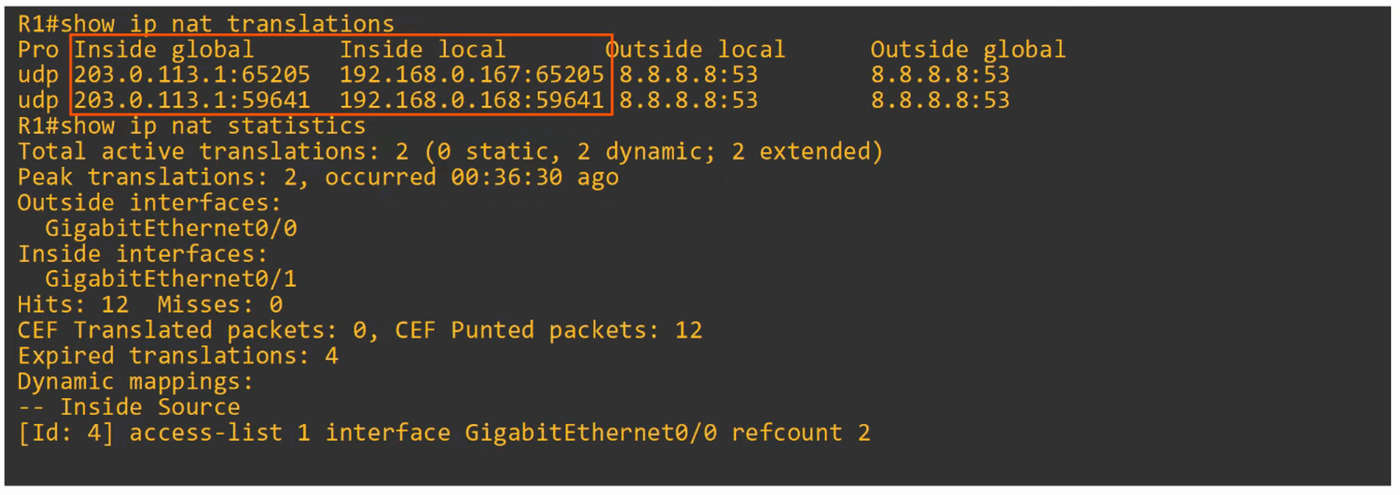
\includegraphics[keepaspectratio,alt={image}]{images/46-nat-dynamic-part2/img-015.png}}
\end{figure}

\section{Command Review}\label{command-review}

\begin{figure}
\centering
\pandocbounded{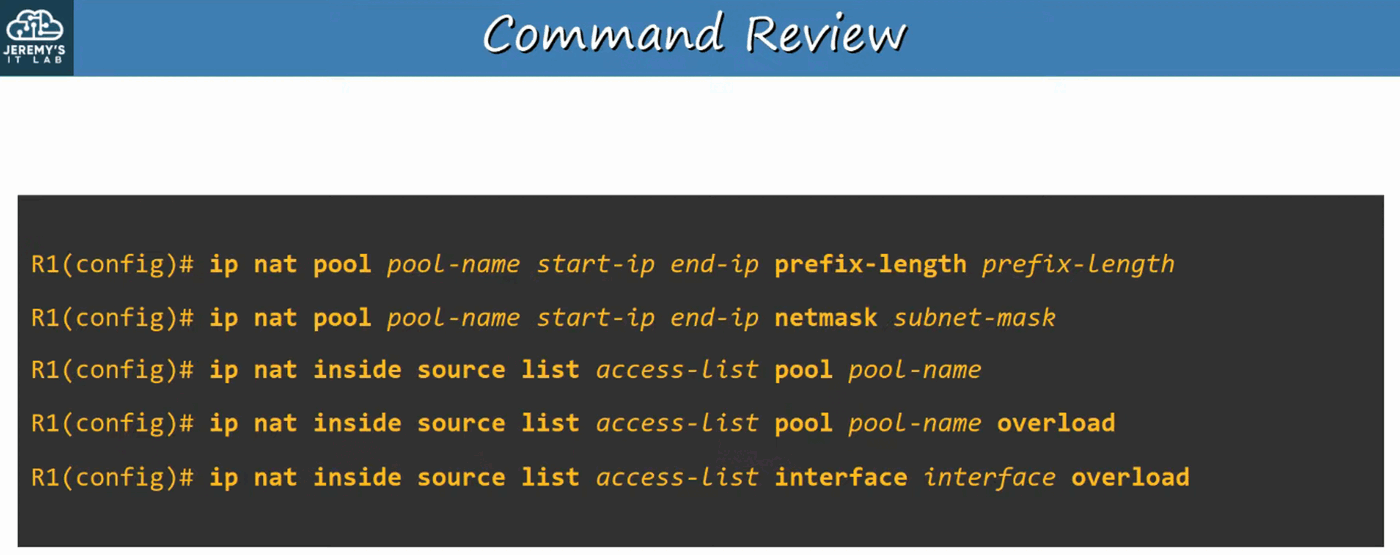
\includegraphics[keepaspectratio,alt={image}]{images/46-nat-dynamic-part2/img-016.png}}
\end{figure}
